	\documentclass{article}
			
		\usepackage{parskip}
		\usepackage{listings}
		\usepackage{xcolor}
		\usepackage{textcomp}
			
		%STYLE AND COLOR DEFINITION FOR SOURCE CODE 	
		\newcommand{\PHPamountofcolor}{75}
		\newcommand{\SourceCodeContext}{5}
		%Lets define the php language colors:
		\definecolor{PHP_comment_old}{HTML}{FF8000}
		\colorlet{PHP_comment}{PHP_comment_old!\PHPamountofcolor!black}
		\definecolor{PHP_default_old}{HTML}{000000}
		\colorlet{PHP_default}{PHP_default_old!\PHPamountofcolor!black}
		\definecolor{PHP_keyword_old}{HTML}{6c9c11}
		\colorlet{PHP_keyword}{PHP_keyword_old!\PHPamountofcolor!black}
		\definecolor{PHP_emph1_old}{HTML}{0F58A2}
		\colorlet{PHP_emph1}{PHP_emph1_old!\PHPamountofcolor!black}
		\definecolor{PHP_emph2_old}{HTML}{CCAA00}
		\colorlet{PHP_emph2}{PHP_emph2_old!\PHPamountofcolor!black}
		\definecolor{PHP_emph4_old}{HTML}{C60484}
		\colorlet{PHP_emph4}{PHP_emph4_old!\PHPamountofcolor!black}
		\definecolor{PHP_string_old}{HTML}{C78F0A}
		\colorlet{PHP_string}{PHP_string_old!\PHPamountofcolor!black}
		\definecolor{PHP_variable_old}{HTML}{C82210}%C82210
		\colorlet{PHP_variable}{PHP_variable_old!\PHPamountofcolor!black}
		\definecolor{PHP_number_old}{HTML}{BF1CA6}
		\colorlet{PHP_number}{PHP_number_old!\PHPamountofcolor!black}
		%Now we want to highlight the variables. This will be done by triggering the function \PHPhighlightvar at the start of any $ run. This function wil only highlight variables and any other identifiers will be ignored. Luckily lstlisting will only give correct identifiers so we only will have to check if the previous call was made with a $
		\usepackage{fontspec}
		\setmonofont{Courier}
		%\usepackage[utf8]{inputenc}
		%\usepackage[T1]{fontenc}
		%\usepackage{courier, textcomp}
		\usepackage{etoolbox}
		\newtoggle{InString}{}% Keep track of if we are within a string
		\togglefalse{InString}% Assume not initally in string
		
		\newcommand*{\ColorIfNotInString}[1]{\iftoggle{InString}{#1}{\color{PHP_number}#1}}%

		%helper
		
		\newcommand{\PHPhighlightvar}[1]{\ifnum\theDollarFlag=1 \color{PHP_variable} \fi#1\setcounter{DollarFlag}{0}}
		\newcounter{DollarFlag}
		
		%images
		\usepackage{graphicx}
		\graphicspath{ {images/} }
		\usepackage{wrapfig}
		\usepackage{subcaption}
		
		
			
			
			
		
			
			\title{Machine Learning: Third Home Work \\ \bigskip \large  KN Neighbors}

			\author{Edoardo Ghini}
			
			\begin{document}
			
			\textbf{\maketitle}
			\pagenumbering{gobble}
			
			\bigskip\bigskip\bigskip
			\begin{center}
			
\includegraphics[width=0.5\textwidth]{laSapienza}
			\end{center}
			\bigskip\bigskip\bigskip
			\textbf{
			Dipartimento di Ingegneria dell'Università di Roma La Sapienza}
			

			\newpage
			\pagenumbering{roman}
			\tableofcontents
			\newpage
			\pagenumbering{arabic}
			
			
			
			
			
			%SETTING STYLE OF SOURCE CODE
			\lstset{
		  language        = php,
		  basicstyle      = \footnotesize\ttfamily,
		  keywordstyle    = \color{PHP_keyword},
		  stringstyle     = \color{PHP_string!90!black}\toggletrue{InString},
		  %this allows highlighting of variables:
		  literate        =  {\$}{{\iftoggle{InString}{\$}{\setcounter{DollarFlag}{1}\color{PHP_variable}\$\color{PHP_default}}}}1
		%    {"}{{{\ProcessQuote{"}}}}1% Disable coloring within double quotes
		%    {'}{{{\ProcessQuote{'}}}}1% Disable coloring within single quote
		    {0}{{{\ColorIfNotInString{0}}}}1
		    {1}{{{\ColorIfNotInString{1}}}}1
		    {2}{{{\ColorIfNotInString{2}}}}1
		    {3}{{{\ColorIfNotInString{3}}}}1
		    {4}{{{\ColorIfNotInString{4}}}}1
		    {5}{{{\ColorIfNotInString{5}}}}1
		    {6}{{{\ColorIfNotInString{6}}}}1
		    {7}{{{\ColorIfNotInString{7}}}}1
		    {8}{{{\ColorIfNotInString{8}}}}1
		    {9}{{{\ColorIfNotInString{9}}}}1,
		  identifierstyle = \color{PHP_default}\PHPhighlightvar,
		  commentstyle    = \color{PHP_comment}\slshape,
		  emph            =[1]{require_once, require, include_once, include, namespace, use, class, function, new},
		  emphstyle       =[1]\color{PHP_emph1},%\bf,
		  emph            =[2]{echo, empty, isset, array, instanceof},
		  emphstyle       =[2]\color{PHP_emph2},%\bf,
		  emph            =[3]{var, const, abstract, 
		                        protected, private, public,
		                        static, final, extends, implements,
		                        global, if, else, foreach ,for,
		                        endforeach, endif, endfor, elseif,
		                        as},
		  emphstyle       =[3]\color{PHP_keyword},%\bf,
		  emph            =[4]{return, throw, exit, __halt_compiler, continue, break},
		  emphstyle       =[4]\color{PHP_emph4},%\bf,
		  breaklines      = true,
		  captionpos      = b,
		  rulecolor       =\color{black},
		  keywords    ={__halt_compiler,    abstract,   and,    array,
		                    as, break,  callable,   case,   catch,  class,
		                    clone,  const,  continue,   declare,    default,
		                    die,    do, echo,   else,   elseif,
		                    empty,  enddeclare, endfor, endforeach, endif,
		                    endswitch,  endwhile,   eval,   exit,   extends,
		                    final,  finally,    for,    foreach,    function,
		                    global, goto, if,   implements, include,
		                    include_once,   instanceof, insteadof,
		                    interface,  isset, list,    namespace,
		                    new,    or, print, private, protected,  public,
		                    require,    require_once, return,   static,
		                    switch, throw,  trait, try, unset, use, var,
		                    while,  xor,    yield,
		  },
		  numbers=left,
		  stepnumber=1,  
		  numberfirstline=true,
		  numberstyle=\footnotesize,
		  xleftmargin=4.0ex,
		  upquote=true,
		  showlines=true
		  }	
			
			\renewcommand{\lstlistingname}{Code}

			
			\part{Introduction}
			
				\section{Scope}
This experience was focused on the comprehension of the theoretic concepts around the classification through KNN algorithm.  
				\section{Objectives}
				The overall assignment was about performing  a classification task on data in fig(1) experimenting various parameters of the KNN classifier like the number of neighbours considered and also experimenting variations about the metric used to compute the distances between points.
				
				\begin{center}
\begin{figure}
\centering
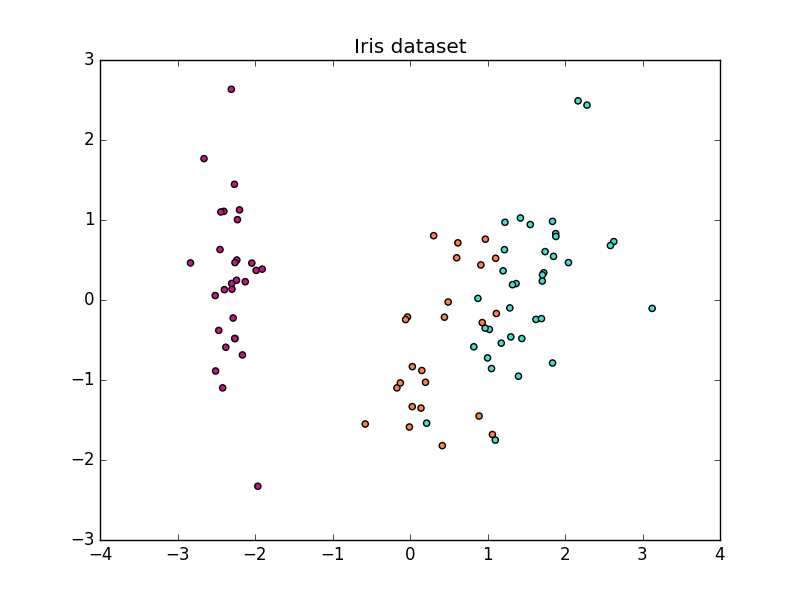
\includegraphics[width=0.9\textwidth]{figure_1}
\caption{}
\label{fig:1}
\end{figure}
\end{center}

\newpage
			\part{Development}
				\section{Data Manipulations}
	
	At first, I loaded the Iris dataset and I standardised the input data. After that, I applied a principal component analysis as common practice to maximise the variance carried from selected data.
	Finally I divided data in test and train subsets.
	
	
	

				\section{Classification}
				As shown in these plots, I performed  the classification of a KNN model with parameters which define the number of neighbours that it would take into consideration assigning the class to new data. This process has been iterated for ten times.
								\begin{center}
				\begin{figure}
\centering
        \begin{subfigure}[b]{0.48\textwidth}
                \centering
                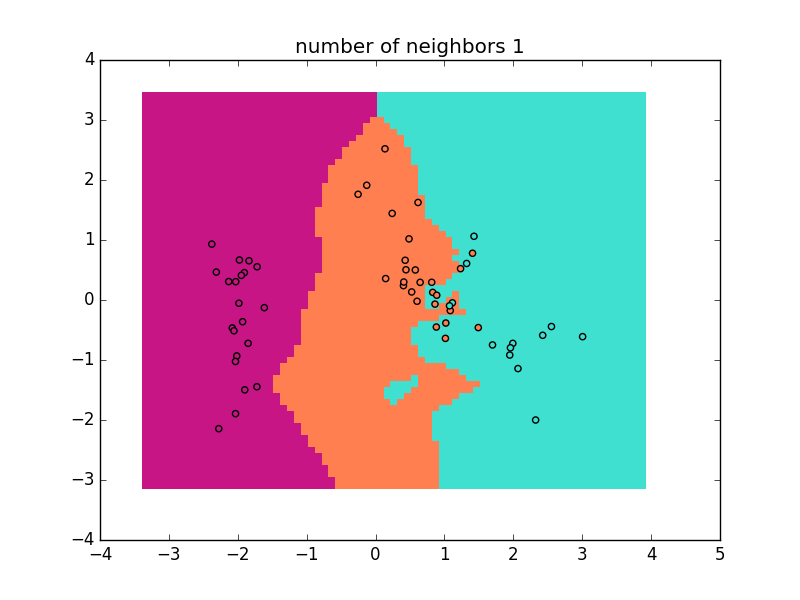
\includegraphics[width=\linewidth]{figure_2}
        \end{subfigure}\hfill
        \begin{subfigure}[b]{0.48\textwidth}
                \centering
                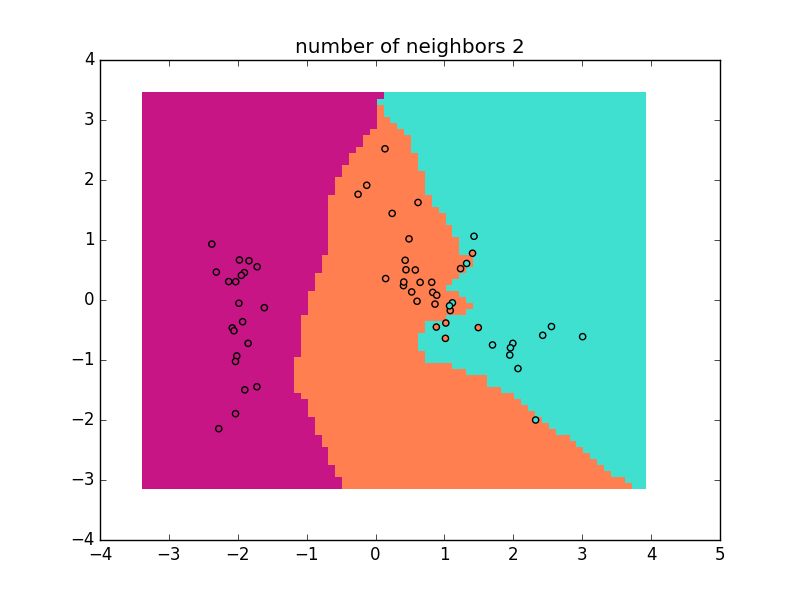
\includegraphics[width=\linewidth]{figure_3}
        \end{subfigure}\hfill
 \label{fig:2}
 \end{figure}
       
\begin{figure}
\centering  
        \begin{subfigure}[b]{0.48\textwidth}
                \centering
                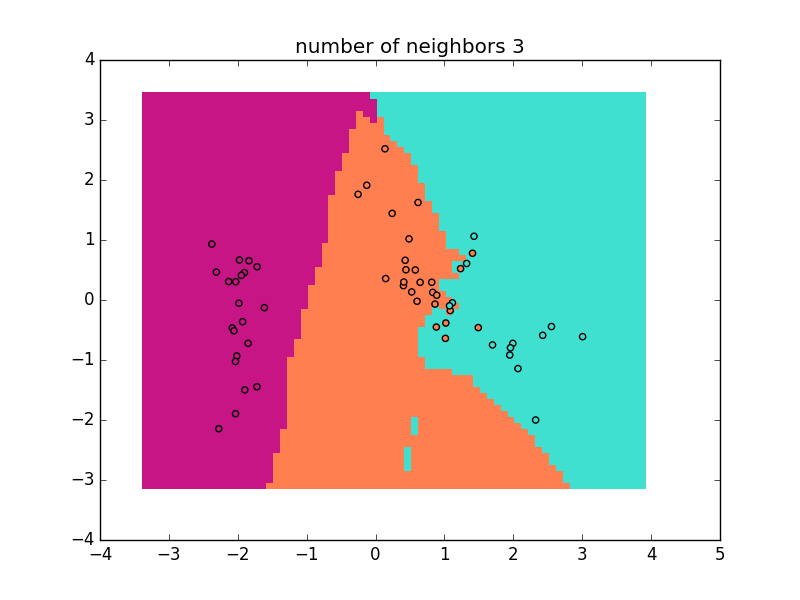
\includegraphics[width=\linewidth]{figure_4}
        \end{subfigure}\hfill
        \begin{subfigure}[b]{0.48\textwidth}
                \centering
                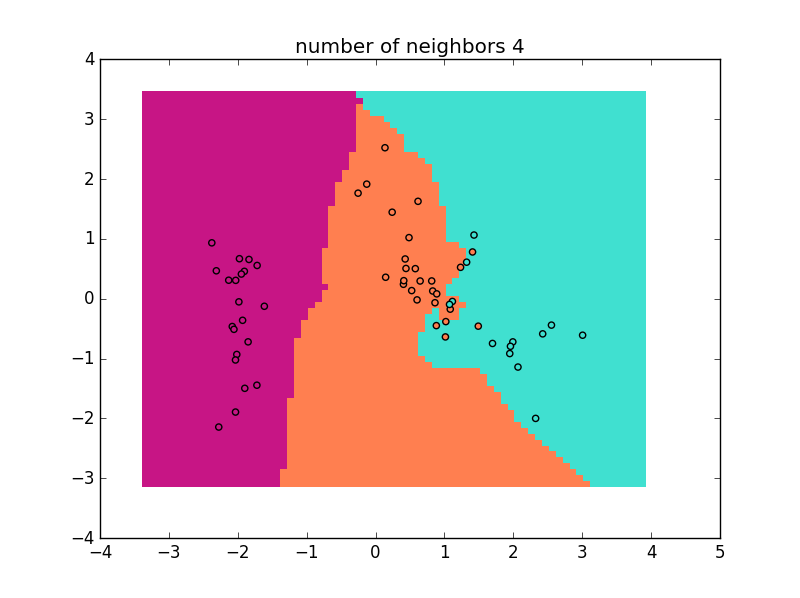
\includegraphics[width=\linewidth]{figure_5}
        \end{subfigure}
        \label{fig:3}
\end{figure}

\begin{figure}
\centering
        \begin{subfigure}[b]{0.48\textwidth}
                \centering
                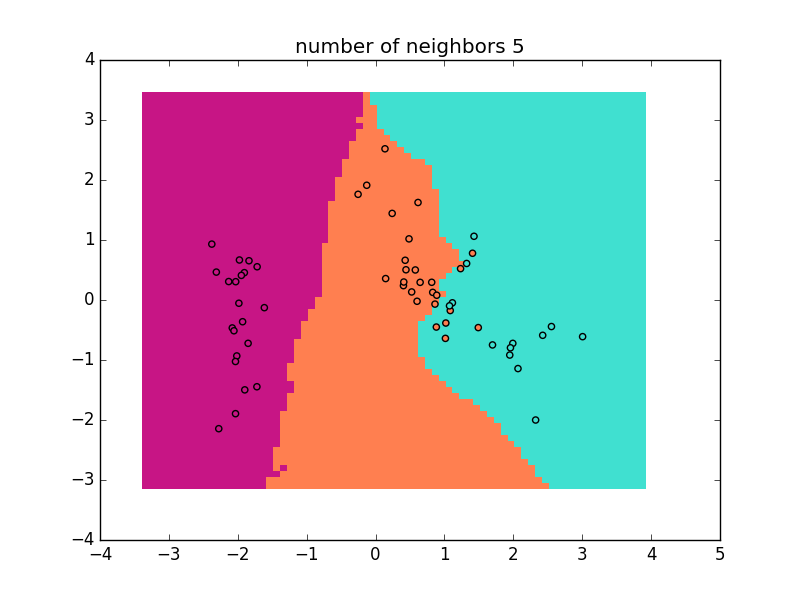
\includegraphics[width=\linewidth]{figure_6}
        \end{subfigure}\hfill
        \begin{subfigure}[b]{0.48\textwidth}
                \centering
                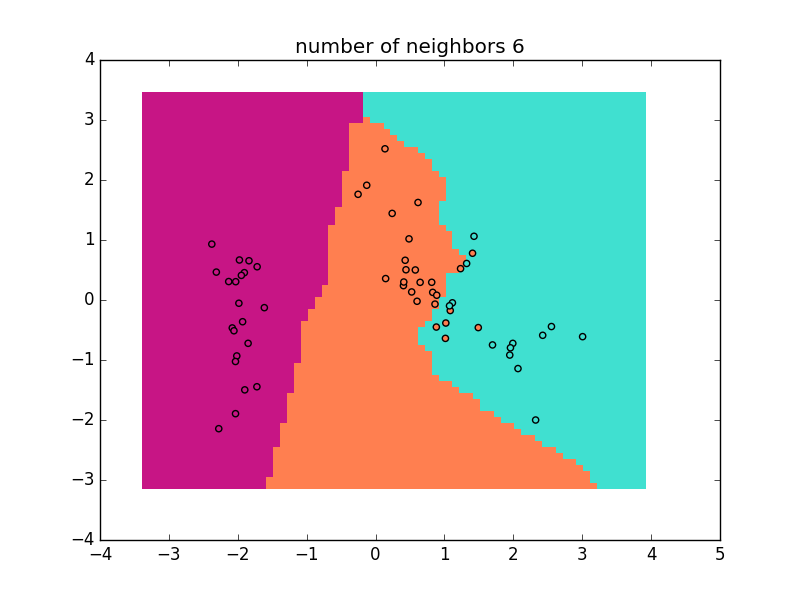
\includegraphics[width=\linewidth]{figure_7}
        \end{subfigure}\hfill
        \label{fig:4}
 \end{figure}
       
\begin{figure}
\centering  
        \begin{subfigure}[b]{0.48\textwidth}
                \centering
                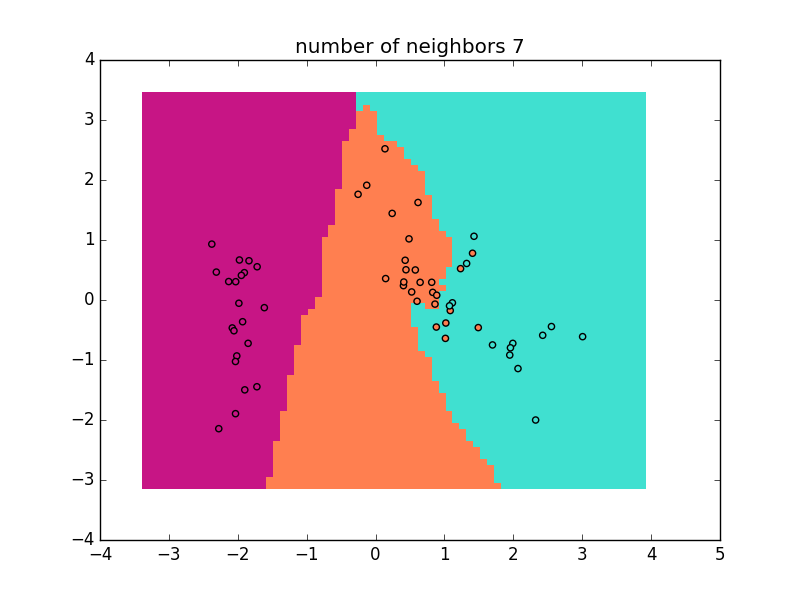
\includegraphics[width=\linewidth]{figure_8}
        \end{subfigure}\hfill
        \begin{subfigure}[b]{0.48\textwidth}
                \centering
                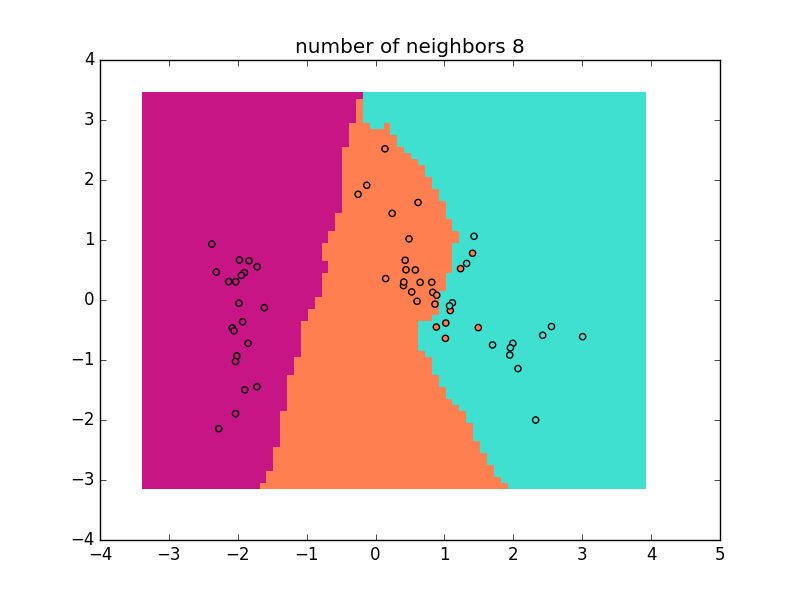
\includegraphics[width=\linewidth]{figure_9}
        \end{subfigure}
        \label{fig:5}
\end{figure}

\begin{figure}
\centering  
        \begin{subfigure}[b]{0.48\textwidth}
                \centering
                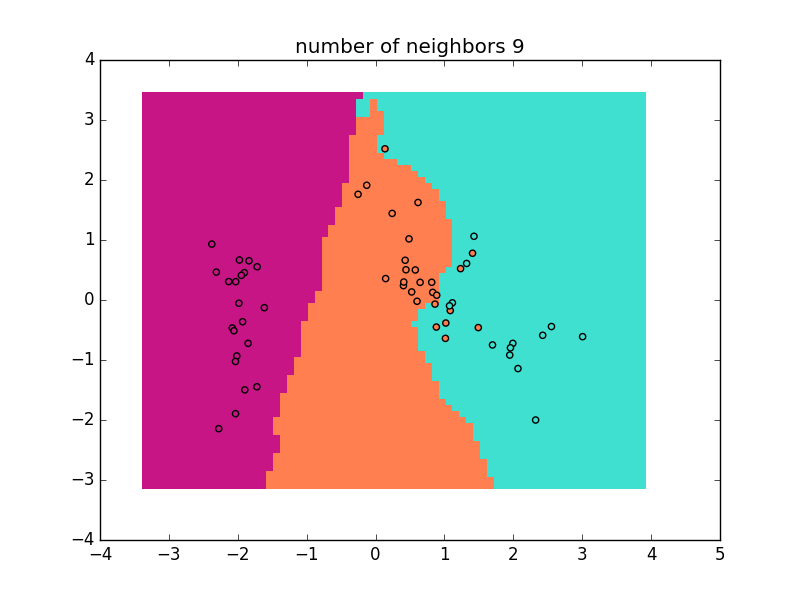
\includegraphics[width=\linewidth]{figure_10}
        \end{subfigure}\hfill
        \begin{subfigure}[b]{0.48\textwidth}
                \centering
                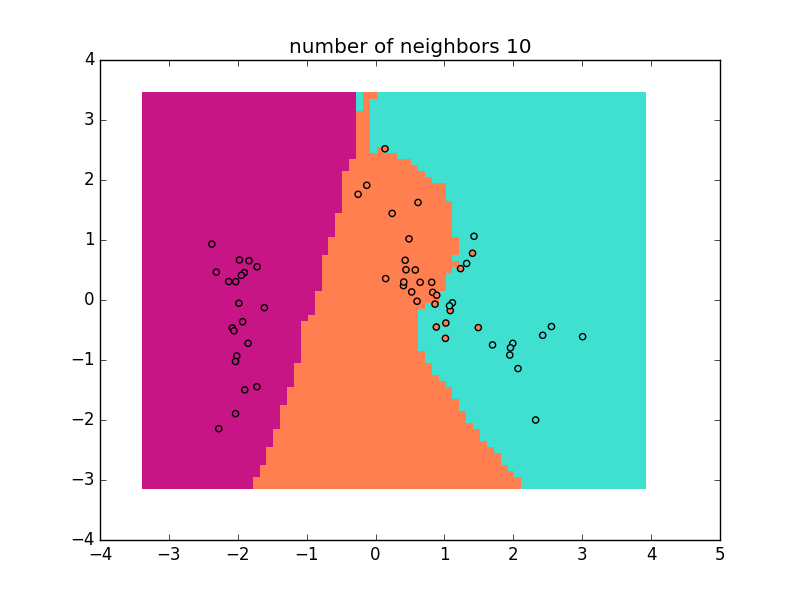
\includegraphics[width=\linewidth]{figure_11}
        \end{subfigure}
        \label{fig:6}
\end{figure}
\end{center}			 
				
				
				
				


				\section{Score Analysis}
				
				In this particular case, with this particular train and test dataset, the best classifier is a KNN that take into consideration three neighbours (fig(7)).
								\begin{center}

\begin{figure}
\centering
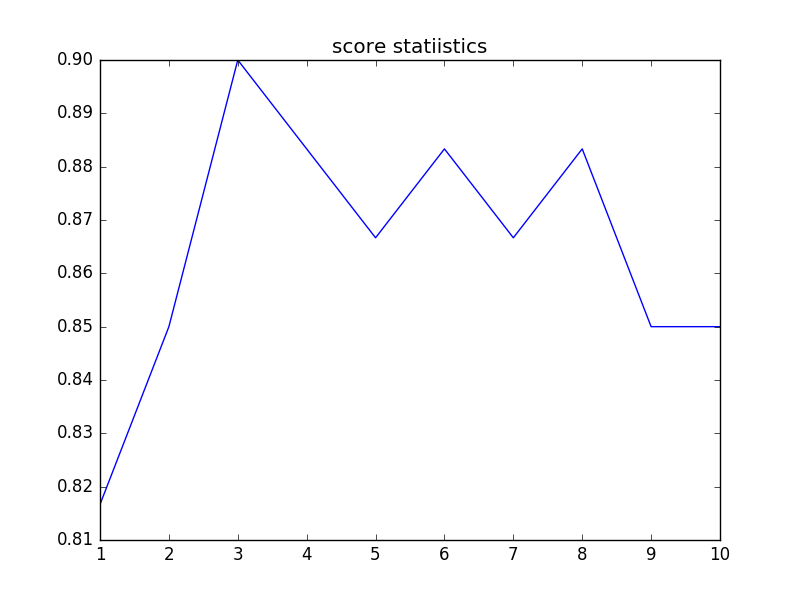
\includegraphics[width=0.9\textwidth]{figure_12}
\caption{}
\label{fig:7}
\end{figure}
\end{center}

				\section{Weights of the Metric}
				By the time, when the best K parameter was found, I tested the classification with two different weight types for distance calculation: in fig(8) is shown the behaviour of weights that consider the euclidean distance between points, instead in fig(9) there is the result due to the adoption of uniform weights so the classification is made on the absolute number of neighbours regardless their distances from the data point that is being classified. 
								\begin{center}

\begin{figure}
\centering
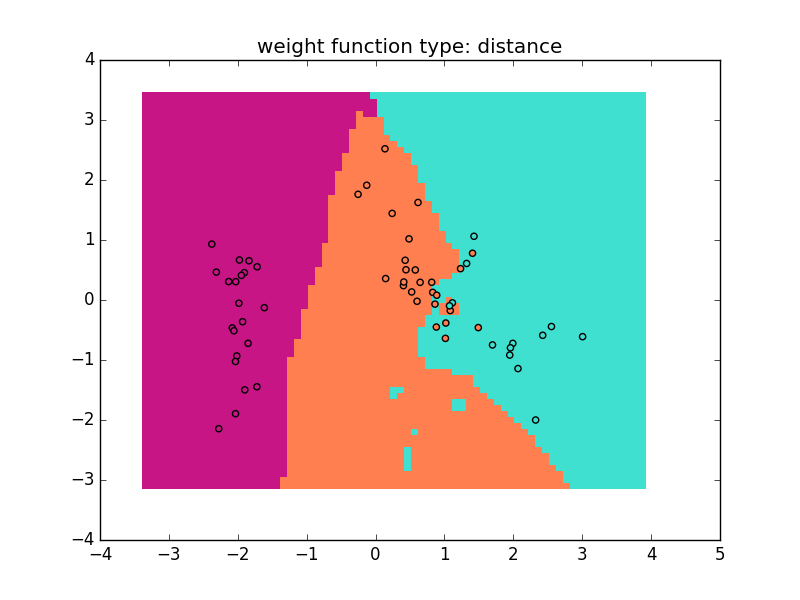
\includegraphics[width=0.9\textwidth]{figure_13}
\caption{}
\label{fig:8}
\end{figure}

\begin{figure}
\centering
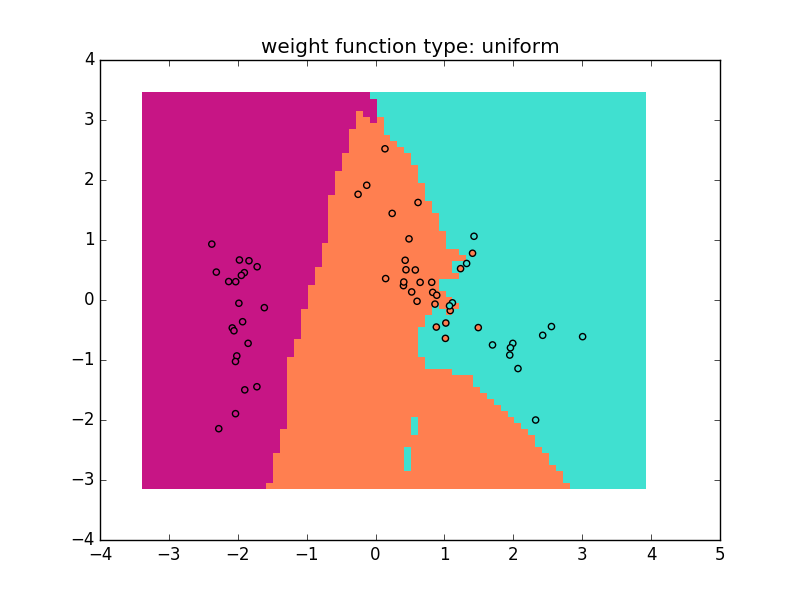
\includegraphics[width=0.9\textwidth]{figure_14}
\caption{}
\label{fig:9}
\end{figure}
\end{center}
				\section{Gaussian Distance Metric}
				Finally I implemented a function on my own in order to compute the distance in a non linear way. These shown below are the results of the classification with the respect of this new metric with different alfa coefficients that affect the steepness of the gaussian function, as it can be seen, in particular, in the last plot with a huge value for alfa
								\begin{center}
				\begin{figure}
\centering  
        \begin{subfigure}[b]{0.48\textwidth}
                \centering
                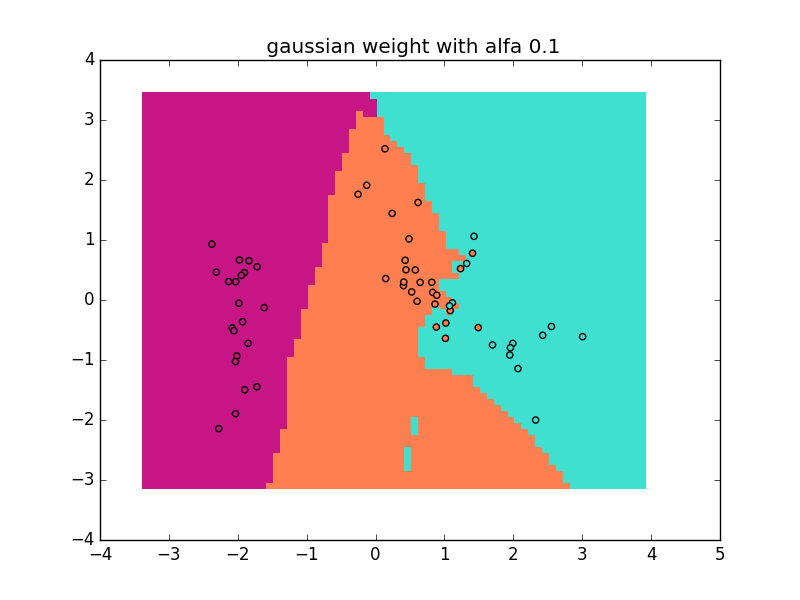
\includegraphics[width=\linewidth]{figure_15}
        \end{subfigure}\hfill
        \begin{subfigure}[b]{0.48\textwidth}
                \centering
                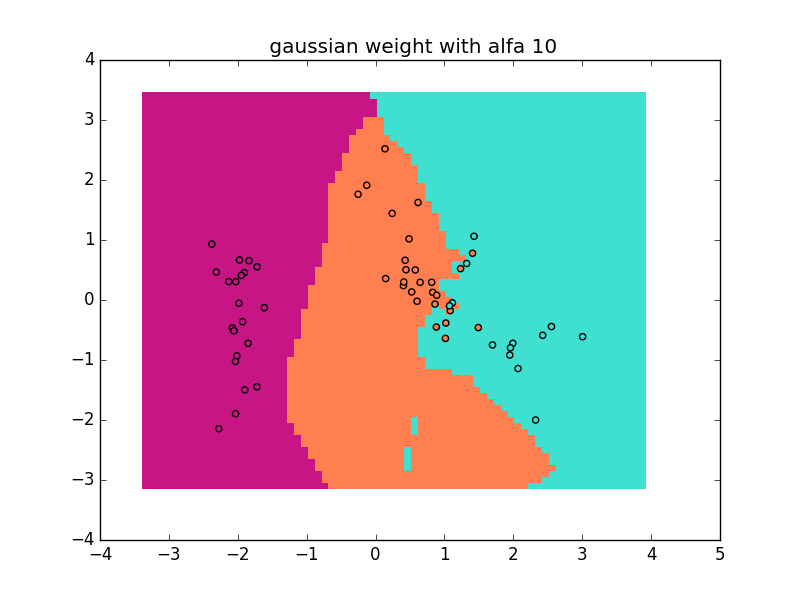
\includegraphics[width=\linewidth]{figure_16}
        \end{subfigure}
        \label{fig:10}
\end{figure}

\begin{figure}
\centering  
        \begin{subfigure}[b]{0.48\textwidth}
                \centering
                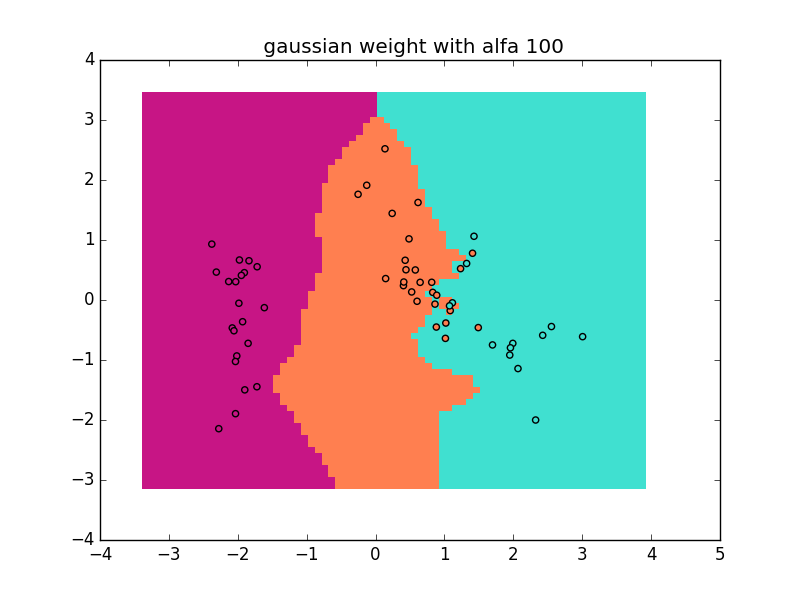
\includegraphics[width=\linewidth]{figure_17}
        \end{subfigure}\hfill
        \begin{subfigure}[b]{0.48\textwidth}
                \centering
                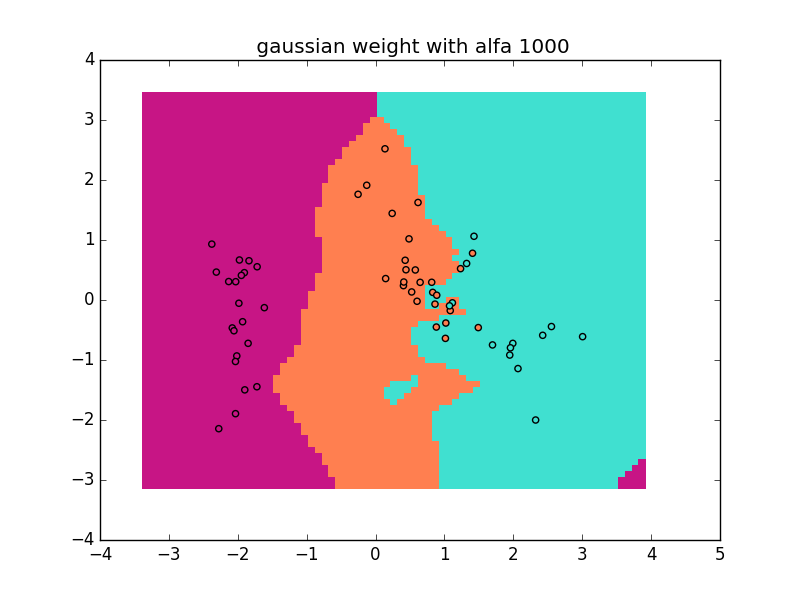
\includegraphics[width=\linewidth]{figure_18}
        \end{subfigure}
        \label{fig:11}
\end{figure}
\end{center}

				
\newpage
			\part{Conclusions}
				
			At the end, collecting the scores of the various classifications, It turned out that for this dataset, the best score around ninety per cent has been achieved with small values of the alfa coefficient.  
			
		\end{document}
